\providecommand{\main}{../../..}
\documentclass[\main/dresen_thesis.tex]{subfiles}
\renewcommand{\thisPath}{\main/chapters/theoreticalBackground/magnetism}
\begin{document}
\section{Magnetism}\label{ch:theoreticalBackground:magnetism}

  Classically, magnetic fields are understood to be produced by moving electric charges \cite{Jackson_1999_Class, Blundell_2001_Magne}.
  Within the framework of special relativity, magnetic fields emerge via a Lorentz transformation from the rest frame of an electric charge to a relatively moving one and the propagation and interaction of the magnetic field with charge and current distributions is fully described by Maxwell's equations.
  A central quantity to describe the sources of magnetic fields is the magnetic moment $\vec{\mu}$, which for localized current distribution $\vec{j}(\vec{r})$ is defined by
  \begin{align}
    \vec{\mu} \eq \frac{1}{2} \int \vec{r} \times \vec{j}(\vec{r}) \dint V .
  \end{align}
  In the case of a closed loop of current $I$, the magnetic moment is just given by the product of the current and the enclosed area $A$, $\mu \eq I A$, with the direction pointing parallel to the surface normal.
  The far-field generated by a magnetic moment is then given by the dipolar field
  \begin{align}
    \vec{B} (\vec{r}) \eq \frac{\mu_0}{4 \pi} \frac{3(\vec{\mu} \cdot \hat{r})\hat{r} - \vec{\mu}}{r^3}.
  \end{align}

  To understand the magnetism of matter, which is generally neutrally charged on the macroscopic scale, the motion of the electrons in the atoms needs to be evaluated\footnote{the direct contribution of the nucleus motion to the magnetism is approximately three orders of magnitude weaker due to the higher mass of the proton and neutrons relative to the electron}.
  The magnetic moment of an electron arises from the spin and orbital motion, which depends on the state the individual particle is in.
  Due to the quantum mechanical nature of the electron, the magnetic moment also needs to be treated quantum mechanically.
  In fact, the Bohr-van-Leeuwen theorem shows that for a purely classical system in thermal equilibrium, the magnetization is always zero.
  The various types of magnetism that are observed within different materials in nature can then be understood by the different structures and the effective couplings of the electrons, which in turn determines the direction of the many magnetic moments within the matter.
  The most popular types that are observed throughout this work are described in the following.

  \subsection{Diamagnetism}
    Diamagnetism is a weak effect that is exhibited by every material and measurable when it is not overshadowed by another type of magnetism.
    When a material enters a magnetic field, Faraday's law of induction states that currents are induced, which by Lenz's law are counter directed to the external field.
    For materials with $n$ electrons per volume, the diamagnetic magnetization can be described quantum mechanically in first order perturbation theory by the Langevin diamagnetism \cite{Blundell_2001_Magne}
    \begin{align}
      M \eq \underbrace{- \frac{n e^2}{6 m_e} \braket{r^2}}_{\eq \chi_D} B,
    \end{align}
    where $\braket{r^2}$ is the mean square distance of the electrons from the nucleus.
    The diamagnetic susceptibility $\chi_D$ is always negative and for common materials $\mu_0 \chi_D$ is in the order of $10^{-5}$.

    In magnetometry experiments, diamagnetism is observed from non-magnetic background materials such as a silicon substrate that carries the actual sample of interest or a solvent.
    As the Langevin diamagnetism is a linear function in $B$ that is largely temperature independent, it can in general be easily separated from other magnetic contributions if it is not negligible in strength.

  \subsection{Paramagnetism}\label{ch:theoreticalBackground:magnetism:paramagnetism}
    Paramagnetism is observed in materials that have atomic or molecular orbitals with unpaired electrons.
    At zero field, if the magnetic moments are localized and decoupled, the direction of the moments is randomly distributed through thermal movement.
    Given an external magnetic field, the magnetic moments of the electrons feel a torque that tries to align the electron moment and field to minimize the Zeeman energy
    \begin{align}
      E_Z = - \vec{\mu}_e \cdot \vec{B}.
    \end{align}
    To determine the magnetization of a paramagnetic material at finite temperature and fields, Boltzmann statistics can be applied to obtain the partition function of the system and from this the magnetization.
    In the classical approach, this leads to the formula for Langevin paramagnetism as shown in \refapp{ch:appendix:calculations:magnetizationClassicalSpin}
    \begin{align}
      M \eq n \mu_e \Biggl( \coth \biggl(\frac{\mu_e B}{k T} \biggr) - \frac{k T}{\mu_e B} \Biggr).
    \end{align}
    For electrons, the energy scale of the Zeeman levels is $\mu_e B \ll kT$ and therefore
    \begin{align}
      M \approx \underbrace{\frac{n \mu_e^2}{3kT}}_{\eq \chi_P} B,
    \end{align}
    which shows that the paramagnetic susceptibility is positive and has a temperature dependance according to the Curie law $M \propto T^{-1}$.

  \subsection{Ferromagnetism, Antiferromagnetism, Ferrimagnetism}
    \begin{figure}[tb]
      \centering
      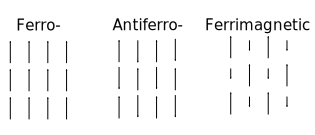
\includegraphics{magnetism_fm_afm}
      \caption{\label{fig:theoreticalBackground:magnetism:fm_afm_fim}Depiction of relative orientation and magnitude of the magnetic moments in a ferro-, antiferro- and ferrimagnetic material.}
    \end{figure}

    When a material has atoms with electrons in an unpaired state nearby to each other, they generally interact for multiple reasons that are touched in the following.
    If the interaction is not negligible, the magnetic moments affect the direction of one another and align mutually along preferred directions.
    \subsubsection{Exchange Interaction}
      A strong quantum mechanical effect between the spin of two electron, the exchange interaction, emerges from the Coulomb interaction and the Pauli exclusion principle.
      Electrons with overlapping states alter their charge distribution by aligning their spins $\vec{S}$ to one another and thus reduce their respective repulsion and the total energy of the system.
      This can effectively expressed by minimizing the exchange energy given by the Heisenberg model
      \begin{align}
        E_{ex} \eq -\sum_{i \neq j} J_{ij} \vec{S}_i \cdot \vec{S}_j,
      \end{align}
      where $J_{ij}$ is the exchange integral that determines the coupling strength between two electron spins.
      Depending on the sign of $J_{ij}$, the energy is minimized by parallel alignment ($J_{ij} > 0$) or anti-parallel alignment ($J_{ij} < 0$).
      The parallel alignment is associated with a ferromagnetic state of the material, whereas the anti-parallel alignment is, when the coupled magnetic moments are of the same magnitude, known as the antiferromagnetic.
      The ferrimagnetic state as depicted in \reffig{fig:theoreticalBackground:magnetism:fm_afm_fim} can be found in mixed compounds, when the anti-parallel aligned moments are not of equal magnitude and therefore a non-zero magnetic moment remains in the net sum.

    \subsubsection{Magnetic Anisotropy}
      Even though the Heisenberg model captures the alignment between magnetic moments, it is isotropic and does not describe observed anisotropies in magnetic materials.
      Due to spin-orbit coupling and dipole-dipole interaction between the electrons, the shape and crystal structure of a material influences the magnetic behaviour and makes some direction in the crystal energetically favorable to another.
      Along this direction, called the easy axis, the magnetization of the material increases stronger than along another direction, whereas the saturation magnetization reached at high fields is independent of the direction.
      The anisotropy can be expressed phenomenological as power series in the directional cosines between the easy-axis and the direction of the magnetization in dependence of the the crystal system.

      In this work, uniaxial and cubic anisotropies are considered.
      The uniaxial system is used to describe a single preferred direction as easy axis or when higher order terms in the anisotropy are negligible.
      If $\theta$ describes the angle between the easy-axis and the magnetization, the anisotropy energy is
      \begin{align}
        E_\mathsf{ani} \eq K V \sin(\theta)^2,
      \end{align}
      with $K$ a material dependent anisotropy constant and $V$ the volume of the material.

      For cubic crystal systems, the anisotropy energy is given by
      \begin{align}
        E_\mathsf{ani} \eq
          \frac{K_1 V}{4} \biggl(\sin(2 \theta)^2 + \sin(\theta)^4 \sin(2\phi)^2 \biggr) +
          \frac{K_2 V}{16} \biggl( \sin(2 \theta)^2 \sin(2 \phi)^2 \sin(\theta)^2 \biggr),
      \end{align}
      where $\phi, \, \theta$ are the angle between the (001) direction and the magnetization direction in spherical coordinates.
      For $K_1 > 0$ and $K_2 > -9 K_1$ the \{100\} directions of the cubic system are the easy axis and for other values either \{110\} or \{111\} are the easy-axis.

    \subsubsection{Magnetostatic Self-Energy}
      An extended magnetic material produces a stray field, which adds a magnetostatic self-energy to the system that counteracts the magnetization.
      The demagnetizing field $\mu_0 \vec{H}_d$ depends on the shape of the magnet and can be calculated for a given sample magnetization $M$ on the mesoscopic scale using the macroscopic Maxwell's equations of magnetostatics and the material equation, which for a current-free magnetic material are \cite{Jackson_1999_Class}
      \begin{align}
        \vec{\nabla} \cdot \vec{B} \eq& 0,\\
        \vec{\nabla} \times \vec{H} \eq& 0,\\
        \vec{B} \eq& \mu_0 (\vec{H} + \vec{M}).
      \end{align}
      As the magnetic field $H$ is curl-free, it can be expressed by a scalar potential $\vec{H} \eq -\vec{\nabla} U$ according to the Helmholtz theorem.
      Using the material equation and plugging both into the divergence-free condition for the magnetic field $B$, the scalar potential is determined by the differential equations
      \begin{align}
        U \eq \begin{cases}
          \vec{\nabla} \cdot \vec{M}, & \vec{r} \in V \\
          0, &\vec{r} \notin V,
      \end{cases}
      \end{align}
      inside and outside of the magnetic material, with the boundary condition that $U$ and normal component of $B$ is continuous at the surface
      \begin{align}
        U_\mathsf{in} &\eq U_\mathsf{out},\\
        \frac{\partial}{\partial n} U_\mathsf{in} &\eq \frac{\partial}{\partial n} U_\mathsf{out} + \vec{M} \cdot \vec{n}.\\
      \end{align}
      The magnetostatic self-energy is then given by the interaction of the magnetization of the material with the demagnetizing field
      \begin{align}
        E_{ms} \eq -\frac{\mu_0}{2} \int_V \vec{M} \cdot \vec{H}_d \dint V
      \end{align}
      To minimize the magnetostatic energy, it becomes above a material dependent crystallite size energetically favorable to create separate domains of regions of coherent spin alignment and therefore vary the magnetization direction across the material.
      The average domain size is then determined by the balance of energy needed to keep the domain walls and the energy gained from minimizing the self-energy.

    The domain formation and the magnetic anisotropy both result in the characteristic hysteretic magnetization behaviour observed for ferromagnetic and ferrimagnetic bulk materials below the order temperature.
    % Upon exposure to a sufficiently strong external magnetic field a hyst, with a remanent magnetization $M_R$ at removal of the field and the need of a coercive field $B_C$ to return the magnetization of the material to zero.

  \subsection{Superparamagnetism}
    When the crystallite size of a ferromagnetic material is reduced, domain formation is no longer energetically favorable below a material dependent size, which is typically in the order of nanometers.
    At this point, the individual electron magnetic moments in the crystallites can align to one another in a single domain and add to a coherent superspin.
\end{document}